\section{Implementierung der Holdback Queue}

Wie bereits in Kapitel \ref{Problemstellungen} erläutert, wird die \textit{Holdback Queue} mit zwei verschiedenen Strukturen implementiert.

Für die Struktur des \textit{HeapSorts} gilt, dass jedes Element die Form \{$[$\textit{Nnr, Msg, TSclientout, TShbqin}$]$, Höhe, linkerTeilbaum, rechterTeilbaum\} hat. Außerdem ist die \textit{Nnr} des Wurzelelements stets kleiner, als die der Kinderelemente. Die beiden Kinderelemente werden nicht miteinander verglichen. Diese Form des Heaps nennt sich \textit{Min Heap} (siehe Abbildung. \ref{fig:binHeap}).

\begin{figure}[htbp]
\begin{center}
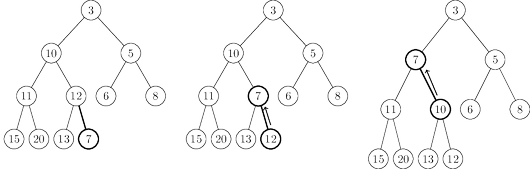
\includegraphics[scale=0.6]{Latex/Bilder/heapExample.png}
\caption[Binary Min Heap Insert]{Binary Min Heap Insert\footnotemark}\label{fig:binHeap} 
\end{center}
\end{figure}
\footnotetext{\url{https://rosalind.info/glossary/algo-binary-heap/}}

Für das Entfernen eines neuen Elements entsteht der Vorteil, dass das Element im Normalfall die Wurzel des Heaps ist, da es die kleinste Nachrichtennummer hat und somit ganz oben als Wurzel gespeichert ist. Beim Einfügen des Elements ist der Heap von Vorteil, da die Elemente ohne erkennbare Sortierung (siehe Abbildung \ref{fig:HBQFilesEntry}) vom Server in den Heap eingefügt werden. Die Elemente werden am höchsten freien Index eingefügt und wandern im Heap nach oben, bis sie ihre korrekte Position erreicht haben. Im Beispiel ist zu sehen, wie das Element mit der Nummer 7 eingefügt wird und solange mit dem Elternknoten getauscht wird, bis dieses größer ist. 

\begin{figure}[htbp]
\begin{center}
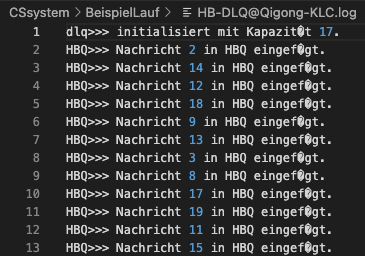
\includegraphics[scale=0.55]{Bilder/HBQFilesEntry.png}
\caption{\label{fig:HBQFilesEntry} Nachrichtendienst \cite{HBQlogging}} 
\end{center}
\end{figure}

Das Konzept des \textit{HeapSort} Algorithmus basiert darauf, dass die neuen Elemente als Blatt eingefügt und die sortierten Elemente als Wurzel entfernt werden. Im \textit{Min Heap} ist das Wurzelelement das kleinste Element des Baums. Dieser wird für die \textit{Holdback Queue} verwendet\footnote{Hierfür wurde der \textit{Max Heap} des zweiten Praktikums in Teilen wiederverwendet.}\footnote{Für weitere Informationen und Entwürfe über die Heap Funktionen siehe Anhang \ref{anhang} und \cite{sortAlgo}.}.

\subsection{initHBQ}

Das Initialisieren der \textit{Holdback Queue} wird durch die Erlang Funktion \textit{spawn/1}, an welche als Parameter die zu startende Funktion übergeben wird, realisiert. Hierbei wird ein neuer Prozess erzeugt und initialisiert. Die ProzessID dieses neu erzeugten Prozesses, wird als Rückgabeparameter in einer Variable gespeichert. 
Die globale Registrierung des Prozesses findet über den Aufruf \textit{register/2} statt. Als Parameter werden zum einen die ProzessID, des zu registrierenden Prozesses übergeben und zum anderen das Atom, unter welchem der Prozess gespeichert werden soll. 
Außerdem wird die Initialisierung der \textit{Delivery Queue} über die \textit{Holdback Queue} aufgerufen. Diesem Aufruf wird der Parameter DLQ-Limit, die maximale Größe der Delivery Queue, mit übergeben. 

Durch Rekursion kann der Status des Prozesses, unter anderem die Informationen über die \textit{Holdback} und \textit{Delivery Queue}, vollständig in den Parametern der Funktion gehalten werden (frei nach \cite{learnErlang}). Der Prozess der \textit{Holdback Queue} wird hierfür über die Funktion \textit{loop} gestartet. Dieser Funktion wird als Parameter die \textit{Holdback Queue} und dessen nächster freier Index oder Größe übergeben. Außerdem die \textit{Delivery Queue} mit maximaler Größe und die logging Datei. Somit können diese über jeden loop Aufruf beschrieben und gelesen werden. 
Ob der nächste freie Index oder die aktuelle Größe übergeben wird, hängt von der Struktur der \textit{Holdback Queue} ab. 

\subsection{checkHBQ} \label{checkHBQ}

Um die Nachrichten der \textit{Holdback Queue} regelmäßig auf Auslieferbarkeit zu prüfen, wurde hierfür eine weitere Funktion implementiert. 
In dieser wird das derzeitige erste Element der \textit{Holdback Queue} (im Folgenden 'SmallestElem') mit der von der \textit{Delivery Queue} erwarteten Nummer ('ExpNrDLQ') verglichen. 
Dadurch wird erkannt, ob Elemente aus der Holdback Queue verworfen oder an die Delivery Queue ausgeliefert werden sollen. 
Zum Beispiel wird im Fall SmallestElem == ExpNrDLQ das SmallestElem an die \textit{Delivery Queue} ausgeliefert. Bei SmallestElem $<$ ExpNrDLQ wird das SmallestElem verworfen, da es nicht mehr benötigt wird und die \textit{Holdback Queue} ansonsten blockieren würde. Benötigt wird es nicht mehr, da die Delivery Queue als aufsteigende Liste ohne Duplikate und ohne fehlende Nachrichtennummern definiert ist. Alle Nachrichten, welche eine kleinere Nachrichtennummer als das aktuell kleinste Element der \textit{Delivery Queue} haben, werden von dieser nicht mehr angefragt und können somit aus der Holdback Queue verworfen werden.  
Für den Fall, dass die Holdback Queue keine Elemente mehr enthält wird eine entsprechende Ausgabe geloggt. 

\begin{figure}[htbp]
\begin{center}
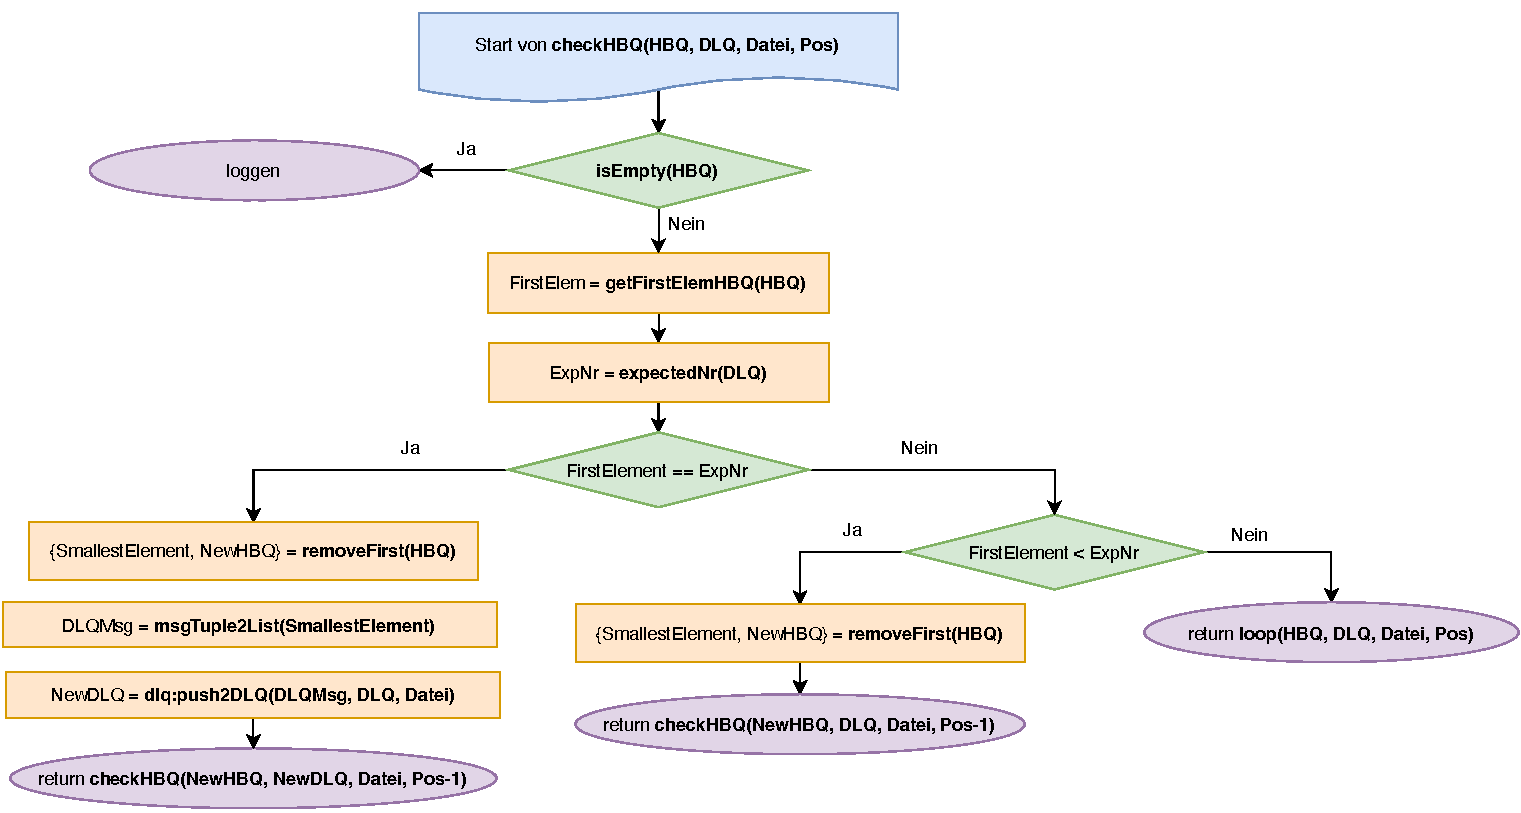
\includegraphics[scale=0.58]{Latex/Bilder/checkHBQ.pdf}
\caption{checkHBQ}\label{fig:checkHBQ}
\end{center}
\end{figure}

Wenn also zum Beispiel nur Elemente größer 3 in die \textit{Holdback Queue} eingefügt wurden, dann fehlen die Elemente 1, 2 und 3 zum Einfügen in die \textit{Delivery Queue}. In der Fehlermeldung steht "Fehlernachricht für Nachrichten 1 bis 3 generiert.". Die 3 wird als Nachricht zusätzlich in die \textit{Delivery Queue} eingefügt.

Die Funktion wird nach jeder Ausführung der \textit{pushHBQ} Funktion aufgerufen. Somit ist sichergestellt, dass nach jeder Veränderung der Queue einmal geprüft wird, ob diese noch synchronisiert ist und keine für die \textit{Delivery Queue} geeignete Nachricht vom Server geschickt wurde.

\subsection{pushHBQ} 

In dieser Funktion wird eine Nachricht in die \textit{Holdback Queue} geschrieben. Die Nachricht enthält die entsprechende Nachrichtennummer und den Inhalt der Nachricht. Außerdem einen Timestamp, wann der Client die Nachricht abgeschickt, bzw. die \textit{Holdback Queue} diese empfangen hat. 

Bedingt durch die fehlende Sortierung der Clients, wird jedes Element als Blatt eingefügt\footnote{Zum Bestimmen des Pfades der nächsten freien Blatts wird wie in der letzten Praktikumsaufgabe die sortv.erl Datei \cite{sortv} verwendet.}. Hier wird als Parameter die Position, also der höchste freie Index, mit übergeben. Dieser muss bei jedem Einfügen eines Elements erhöht und beim Löschen eines Elements um eins verkleinert werden. 

\begin{figure}[htbp]
\begin{center}
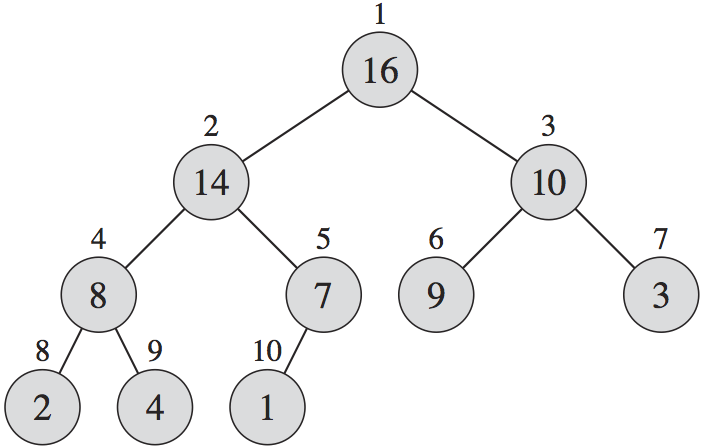
\includegraphics[scale=1]{Latex/Bilder/heapIndex.png}
\caption[Binary Heap Index]{Binary Heap Index\footnotemark}\label{fig:binHeapIndex}
\end{center}
\end{figure}
\footnotetext{\url{https://weibeld.net/algorithms/data-structures.html}}

\newpage

\begin{lstlisting}
% sortv.erl
% @author: Prof Dr Christoph Klauck, HAW Hamburg 
calcPath(Number) -> calcPath(Number,[]).
% aktuelle Position ist Wurzel
calcPath(1,Accu) -> Accu;
% aktuelle Position ist gerade
calcPath(Number,Accu) when Number rem 2 =:= 0 -> calcPath(Number div 2,[l|Accu]);
% aktuelle Position ist ungerade
calcPath(Number,Accu) when Number rem 2 =/= 0 -> calcPath((Number-1) div 2,[r|Accu]).	
\end{lstlisting}

Anhand dieses Indexes kann der Pfad durch modulo Rechnungen bestimmt werden. Wird wie im Beispiel in der Abbildung \ref{fig:binHeapIndex} eine ungerade Position, in diesem Fall die 11, übergeben, wird der Pfad \textit{$[l|r|r]$} zurückgegeben. Es müssen also zuerst der linke Teilbaum und dann zweimal der rechte Teilbaum gewählt werden, um in das nächste freie Blatt zu gelangen.
Die Position des höchsten Index wird als Integer zusammen mit der Holdback Queue als Parameter in der loop Funktion mit übergeben und somit rekursiv gespeichert. 

Bedingt durch die limitierte \textit{Delivery Queue} Größe, wird der Inhalt der \textit{Holdback Queue} ab einer erreichten Größe von $\frac{2}{3}*sizeOf(DLQ)$ reduziert. Dafür wird geprüft, wie groß die Lücke zwischen den beiden Queues ist. Ein Beispiel dafür ist in Abbildung \ref{fig:BeispielHBQFehler} zu sehen. Hier hat die \textit{Holdback Queue} diese bestimmte Größe erreicht und die Lücke in der \textit{Delivery Queue} wird dementsprechend aufgefüllt. Aufgefüllt werden hierbei nicht alle fehlenden Nachrichten, sondern nur die von der \textit{Delivery Queue} zuletzt erwartete. Eine ähnliche Fehlermeldung wie in der Abbildung wird in Textform in diese Nachricht als \textit{Msg} eingetragen. 

\begin{figure}[htbp]
\begin{center}
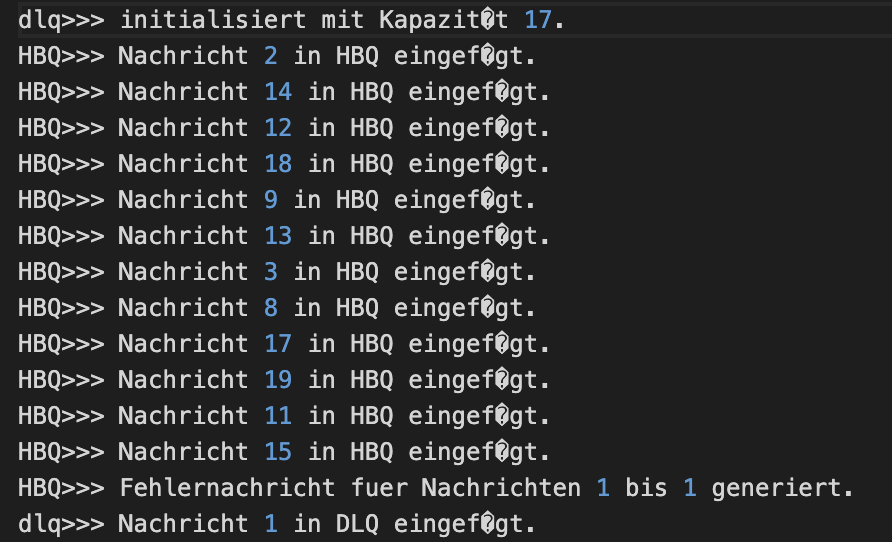
\includegraphics[scale=0.6]{Bilder/BeispielHBQFehler}
\caption{\label{fig:BeispielHBQFehler} Fehlermeldung Beispiel \cite{HBQfehler}} 
\end{center}
\end{figure}

Die Elemente, welche aus der \textit{Holdback Queue} an die \textit{Delivery Queue} gesendet wurden, werden aus der \textit{Holdback Queue} gelöscht, da ansonsten die Größe der Queue nicht aktualisiert werden kann. 

Ein weiteres Problem entsteht, wenn Elemente eingefügt werden, welche eine kleinere Nachrichtennummer haben als das zu erwartende nächste Element der \textit{Delivery Queue}. \\
In diesem Falle wird die einzufügenden Nachricht verworfen und es wird NNr<expNrDLQ an den Prozess gesendet, welcher in der \textit{Holdback Queue} gespeichert ist.

\subsection{deliverMSG}

In dieser Funktion wird die \textit{Delivery Queue} über die \textit{Holdback Queue} beauftragt die zu der übergebenen Nachrichtennummer zugehörige Nachricht zu senden. Der Client welcher die Nachricht empfangen soll wird als ProzessID mit im Parameter der Funktion übergeben. 
Über den Funktionsaufruf \textit{dlq:deliverMSG(MSGNr, ClientPID, Queue, Datei)} wird also die entsprechend zu sendende Nachrichtennummer, die ProzessID, die Delivery Queue und die in die zu loggende Datei übergeben. 
Wenn die übergebene Nachricht nicht verfügbar ist, dann wird die Nachricht mit der nächst größeren Nummer gesendet. 
Als Antwort sendet der Prozess der\textit{ Holdback Queue} die gesendete Nachrichtennummer. 

\subsection{listADT}

Diese Funktion ist aufgeteilt in zwei Funktionen: \textit{listHBQ} und \textit{listDLQ}. 
Es wird in beiden der Inhalt der jeweiligen Queue ausgegeben. Dabei wird die Reihenfolge der Queue beibehalten. Ausgegeben werden alle enthaltenden Nachrichtennummern in Form einer Liste. 

\paragraph{listHBQ}
Für diese Funktion wird über alle Elemente der \textit{Holdback Queue} iteriert und jeweils die Nachrichtennummer in eine separate Liste geschrieben. 
Da die \textit{Holdback Queue} in einer Heap Struktur umgesetzt ist, gibt es zwei mögliche Sortierungen. Zum einen könnte nach Index sortiert werden. Dementsprechend würde das Wurzelelement als erstes ausgegeben werden, dann alle Elemente mit der nächst kleinsten Höhe von links nach rechts gelesen usw..
Die andere Möglichkeit wäre es den Heap bei der Ausgabe zu sortieren. Dafür wird das Wurzelelement als erstes ausgegeben werden, vor der nächsten Ausgabe wird dann erst der Heap neu strukturiert. Das Element mit dem höchsten Index wird die neue Wurzel. Dieses versickert so lange nach unten, bis es keinen kleineren Teilbaum mehr hat. Erst danach wird das nächste Element (also wieder die Wurzel) ausgegeben. 
Der Vorteil der Index-Sortierung ist die kleinere Laufzeit, da im Vergleich zur Nachrichtennummer-Sortierung nicht nach jeder Ausgabe neu strukturiert werden muss. Allerdings sind bei der Index-Sortierung die Nachrichtennummern in der Ausgabe zufällig, was zum Beispiel das händische Finden eines Elements aufwändiger macht. 
Da die Funktionalität in diesem Falle im Vordergrund steht, wird bei \textit{listHBQ} eine Liste in aufsteigend sortierter Reihenfolge ausgegeben. 

Die Ergebnisse werden in eine log Datei geschrieben und bei Erfolg wird als Rückgabewert \textit{ok} als Antwort gesendet.

\paragraph{listDLQ}
Die bereits existierende Funktion \textit{listDLQ} der Delivery Queue, wird hier verwendet. 
Als Queue wird die in der \textit{Holdback Queue} gespeicherte \textit{Delivery Queue} übergeben und die zurückgegebene Liste wird dann in die Logging Datei geschrieben. 

\subsection{dellHBQ}

Um die \textit{Holdback Queue} zu löschen, muss durch die rekursive Implementierung die Funktion loop/4 beendet werden. Dadurch, dass diese Funktion als Schleife implementiert ist, wird durch den Funktionsaufruf \textit{dellHBQ} die Abbruchbedingung simuliert. Nach diesem Aufruf sind dann weder die Elemente innerhalb der Queue noch vorhanden, noch ist die Prozess ID der Queue weiterhin referenziert. 
Außerdem wird das Löschen der \textit{Delivery Queue} von dieser Funktion initialisiert. 

